
\section{Architektur}
\label{Architektur}

In diesem Kapitel wird die Architektur unserer Applikation und die Schnittstellen zu den Umsystemen besprochen. Als Anhaltspunkt wird das C4 Modell \cite{c4model} von Simon Brown verwendet. In einem ersten Schritt wird unsere Applikation in den Kontext des grösseren Systems gesetzt. Anschliessend teilen wir das System \code{TODO} in einzelne Container und den zentralen Container \code{TODO} in einzelne Komponenten auf.

\subsection{Systemkontext}
\label{Architektur:Systemkontext}

In Abbildung \ref{fig:system-context-diagram} ist gestrichelt eingerahmt das System "ÖV-Güteklassen" zusammen mit den dazugehörigen Umsystemen dargestellt. Die Pfeile bedeuten, dass ein System in Richtung der Pfeilspitze Anfragen an ein anderes System sendet. Die Daten fliessen dementsprechend in die entgegengesetzte Richtung.

\begin{figure}[ht]
    \centering
    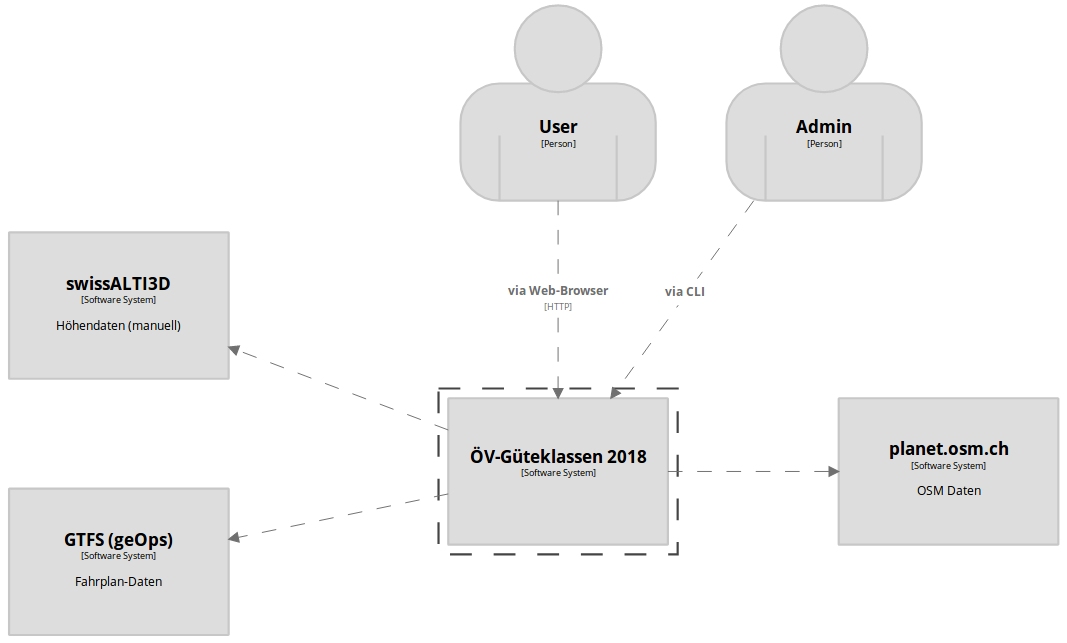
\includegraphics[width=1\linewidth]{projectdoc/img/systemcontext-diagram.png}
    \caption[Systemkontextdiagramm]{Systemkontextdiagramm ÖV-Güteklassen 2018}
    \label{fig:system-context-diagram}
\end{figure}

Im Folgenden werden die Umsysteme sowie die Beziehungen zu unserem System ''Öv-Güteklassen 2018'' genauer beschrieben.

\subsubsection{Web-App}
\label{subsystem:Web-App}

Die Web-App dient zur Darstellung der ÖV-Güteklassen in einer interaktiven Karte für den Benutzer. Dazu erhält es die vorberechneten Daten vom System ''ÖV-Güteklassen 2018'' und visualisiert sie für die Anzeige im Webbrowser.

\subsubsection{swissALTI3D}
\label{subsystem:swissALTI3D}



\subsubsection{GTFS}
\label{subsystem:GTFS}

% TODO
\subsubsection{planet.osm.ch}
\label{subsystem:planet.osm.ch}

% TODO


\subsection{Container}
\label{Architektur:Container}

%TODO


\subsection{Component}
\label{Architektur:Component}

%TODO

\subsection{Code}
\label{Architektur:Code}

%TODO vlt. auf anderes Kapitel verweisen